\chapter{システムの線形性検証とその同定}
\label{sec:SystemIdentification}
対象とするシステムの正確なモデルが得られる場合には,シリンダにかかる力を直接測定することなく他のセンサの値から推定することができる.
前章で導出した物理モデルに基ずけばモデルの構築は可能であるが,バルクや粘性項などのパラメータは温度や圧力などに依存しており,これらの未知のパラメータを正確に同定してモデル化することは現実的に難しい.

そこで本章ではシステム同定を用いて油圧システムのモデル構築を行う.
システム同定では着目するシステムの入出力関係を用いるため,未知パラメータのひとつひとつを場当たり的に同定する必要がないという利点がある.
そこで,本論文では,バルブへの電圧入力からシリンダ先端の位置及び先端で発生する力までのモデルをシステム同定を用いて導出する.
力の同定ではシリンダ先端を固定した状態で同定を行い,位置の同定は先端を固定しない無負荷状態で行う.
%同定にあたってはシステムの周波数応答を調べて特徴を把握したのちに最小自乗法によるモデルの同定,およびM系列を用いた同定を行いそれぞれを比較する.
\section{実験機とその構成}
本論文で開発した油圧システムの実験装置を\figname\ref{fig:ExperimentSystem}に示す.
本装置は片ロッドの油圧シリンダ,ギヤポンプ,サーボバルブなどにより構成されており,シリンダにはロッドの位置を測定するワイヤー式エンコーダおよび,対象物に押し付ける力を測定するロードセルが取り付けてある.
また,圧力センサをサーボバルブのAポートおよびBポート,そしてシリンダのヘッド側とロッド側の入り口の計4箇所に取り付けてある.
シリンダの先端は\figname\ref{fig:stateofsystem}に示すように,力の同定を行うときには固定板へ固定し\figname\ref{fig:State_fixed},位置の同定時には自由に動く状態\figname\ref{fig:State_free}にしている.
\begin{figure}[t]
    \centering
        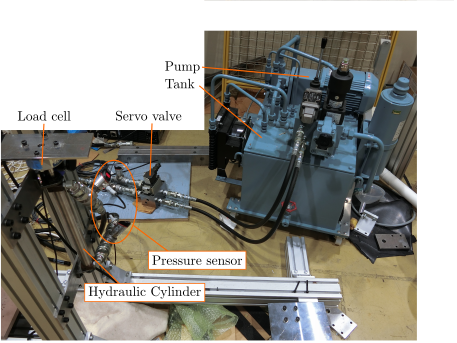
\includegraphics[keepaspectratio, scale=1.0]{contents/SystemIdentification/figure/ExperimentSystem.png}
        \caption{Experiment System}
        \label{fig:ExperimentSystem}
\end{figure}

\begin{figure}[t]
    \begin{minipage}{\minipageratio\hsize}
    \centering
        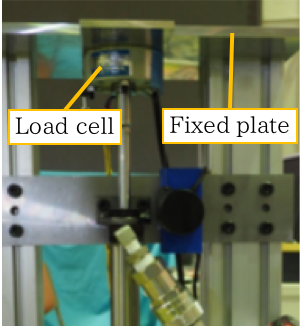
\includegraphics[keepaspectratio, scale = 1]{contents/SystemIdentification/figure/State_fixed.png}
        \subcaption{Fixed}
        \label{fig:State_fixed}
    \end{minipage}
    \begin{minipage}{\minipageratio\hsize}
    \centering
        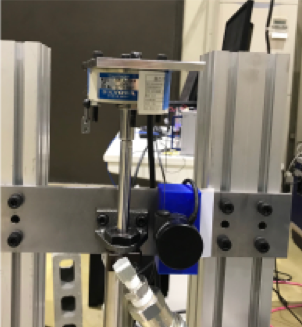
\includegraphics[keepaspectratio, scale = 1]{contents/SystemIdentification/figure/State_free.png}
        \subcaption{Position}
        \label{fig:State_free}
    \end{minipage}
    \caption{State of the Cylinder Tip}   
    \label{fig:stateofsystem}
\end{figure}



コントローラ側はPC及びAD/DA変換器やカウンタで構成されており,実験装置に取り付けてあるセンサからの値の取得及びサーボバルブへの入力を行うことができる.
センサ値の処理やサーボバルブへの入力をするための制御アルゴリズムはPC上でMATLAB/Simulinkを用いて組んでいる.
また,取得したセンサ値に対しローパスフィルタとして$1/(0.005s+1)$を作用させている.
システムの伝達経路の全体像は\figname\ref{fig:ConnectionDiagram}のようになる.
また,本装置に用いている各部品の諸元をTable~\ref{tab:configuration-parameter}にまとめる.

\begin{figure}[t]
    \centering
        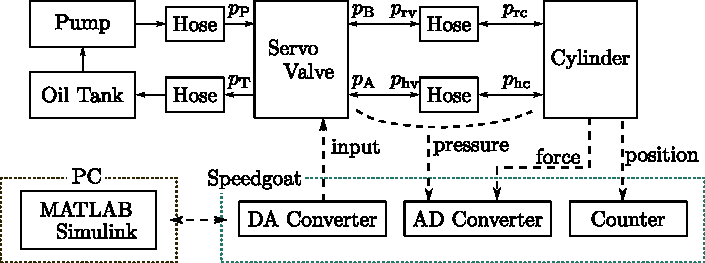
\includegraphics[keepaspectratio, scale=1.0]{contents/SystemIdentification/figure/structionofsystem.pdf}
        \caption{Connection Diagram of the Hydraulic System }
        \label{fig:ConnectionDiagram}
\end{figure}

\begin{landscape}
\begin{table}[t]
    \caption{Experiment System Configuration}
    \label{tab:configuration-parameter}
    \centering
    \begin{tabular}{cccc}
        \hline
        Name & Maker & Model Number & Property\\ \hline \hline
        Servo Valve & nachi & J869-1000A & --- \\
        Hydraulic Cylinder & SMC & CHN-25-250 &     \begin{tabular}{l}internal diameter: \SI{25}{mm} \\ rod diameter: \SI{12}{mm}\end{tabular}\\
        Gear Pump & --- & --- &rated power\SI{7}{Mpa},\SI{2}{l/min} \\
        Oil&\begin{tabular}{l}JXTG Nippon Oil \& \\Energy Corporation\end{tabular}&Super Hyrando 32&--- \\\hline
        Load Cell & KYOWA & LUK-A-10kN & ---\\
        Pressure Sensor & KEYENCE & GP-M250 & --- \\
        Encoder & Micro Tech Laboratory & & --- \\ \hline
    PC & mouse computer & --- & \begin{tabular}{l}cpu:i7-7900K \\ gpu:\\OS:windows 10 education\end{tabular} \\
    \begin{tabular}{l}AD/DA Converter \\ Counter\end{tabular}
    & Speedgoat & Speedgoat & --- \\ 
    MATLAB/Simulink & MathWorks & 2018b & --- \\ \hline \hline
    \end{tabular}

\end{table}
\end{landscape}

\section{先端で発生する力までの線形性とモデルの同定}
\label{sec:力までの同定}
バルブへの入力から先端で発生する力までのシステム同定にあたり,\figname\ref{fig:ConnectionDiagram}に示した伝達経路を入力と内部でやりとりされる力に着目し,\figname\ref{fig:system_dentatsu}のように書き直す.
$\mathrm{input}$はコントローラからバルブへの電圧指令,$\fthr$はシリンダの圧力および受圧面積より算出される推力\footnote{本論文においては,摩擦などを考慮せず圧力と受圧面積のみから算出される力を「推力」とよんでいる.文献により呼び方は様々であるため,注意が必要である.},$f_\mathrm{output}$は実際に先端で発生する力である.
\figname\ref{fig:ConnectionDiagram}は,バルブへの入力によりシリンダを動かそうとする推力$\fthr$が生まれ,$\fthr$が摩擦などの影響を受けて最終的に出力$f_\mathrm{output}$となって出てくるということを表す.
推力$\fthr$は\eqnname\eqref{eq:fthr}により算出される.
\begin{align}
    \label{eq:fthr}
    \fthr = \Ah  \phs - \Ar \prs
\end{align}
ここで$\Ah$はヘッド側の受圧面積,$\Ar$はロッド側の受圧面積,$\phs$はシリンダのヘッド側の圧力,$\prs$はシリンダ側のロッド側の圧力である.
なお,先端で発生する力とはロードセルにより測定された実測値であり,今後これを実測出力と呼ぶ.
\begin{figure}[t]
    \centering
        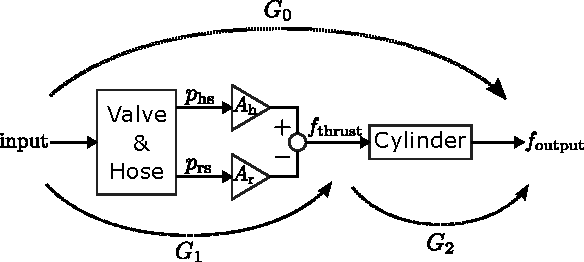
\includegraphics[keepaspectratio, scale=1.0]{contents/SystemIdentification/figure/system_dentatsu.pdf}
        \caption{Diagram for System Identification}
        \label{fig:system_dentatsu}
\end{figure}

\subsection{線形性の検証}
\label{sec:線形性調査(力)}
バルブへの入力に対するシステムの物理量の応答の線形性について調べ,システムの特性の把握を行う.
対象とする物理量は,実測出力$\fmsr$およびシリンダに取り付けてあるヘッド側圧力$\phs$,ロッド側圧力$\prs$である.

バルブへ正弦波入力を与えた際の応答をフーリエ変換したとき,そのピークが入力した正弦波の角速度と一致し,かつその他の角速度でピークが立たない場合に,着目したシステムの入力から出力までは線形応答とみなすことができる.
実験では,バルブへ入力する角速度として\SI{0.1778}{rad/s}から\SI{100}{rad/s}まで対数上で等間隔に12等分したものを採用した.
サンプリング周期は\SI{0.001}{s}であり,センサから取得される値にはローパスフィルタ(以降LPF)として一次遅れの伝達関数${1}/(0.005s+1)$を通している.
また,フーリエ変換を施す前に直流成分を除去し,角速度のピークに着目するため,最大ピークで除すことで正規化している.

各物理量の応答を\figname\ref{fig:1018FFT_fmeasure}から\figname\ref{fig:1018FFT_prs}に示す.
これより最大ピークの角速度と入力した正弦波の角速度が一致しているため,これらの物理量の応答はおおむね線形であるとみなすことができる.
よって,以後対象とする油圧システムは線形なシステムとみなして同定を行うとする.
\begin{figure}[t]
    \centering
        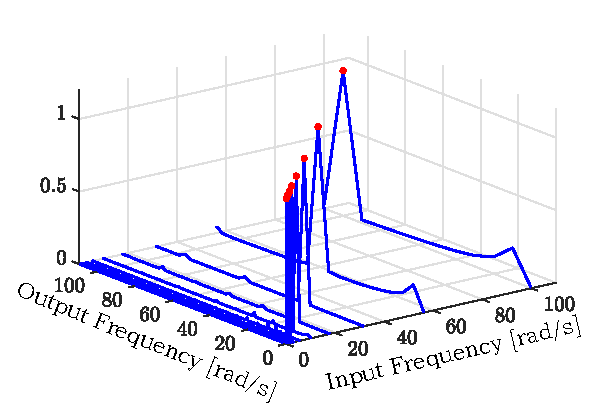
\includegraphics[keepaspectratio, scale=1.0]{contents/SystemIdentification/figure/1018FFT_fmeasure.pdf}
        \caption{FFT of $\fmsr$}
        \label{fig:1018FFT_fmeasure}
\end{figure}
\begin{figure}[t]
    \centering
        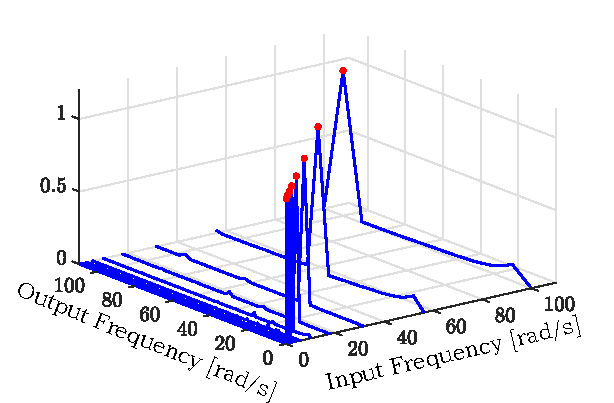
\includegraphics[keepaspectratio, scale=1.0]{contents/SystemIdentification/figure/1018FFT_phs.pdf}
        \caption{FFT of $\phs$}
        \label{fig:1018FFT_phs}
\end{figure}
\begin{figure}[t]
    \centering
        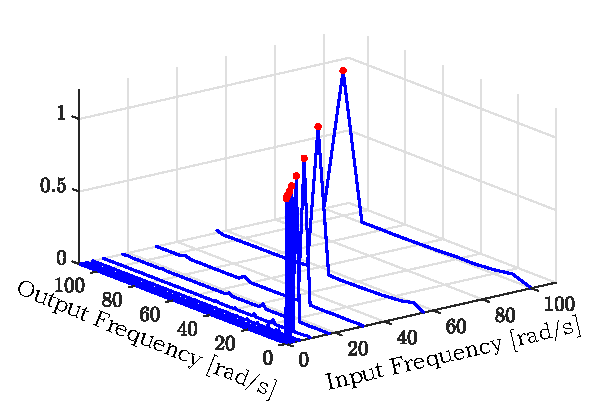
\includegraphics[keepaspectratio, scale=1.0]{contents/SystemIdentification/figure/1018FFT_prs.pdf}
        \caption{FFT of $\prs$}
        \label{fig:1018FFT_prs}
\end{figure}


\subsection{周波数領域における伝達関数モデルの同定}
\label{sec:LD伝達関数モデル(力)}
入力から実測出力$\fmsr$および推力$\fthr$までのシステムを同定するにあたり,はじめに周波数応答を調べ,システムの特性を把握する.
%入力から実測出力までの周波数応答を調べてシステムの特性を把握し,最小ジオ傑法により伝達関数モデルの同定を行う.
バルブへの入力に\ref{sec:線形性調査(力)}節と同様に正弦波入力を角速度を\SI{0.1778}{rad/s}から\SI{100}{rad/s}まで対数上で等間隔に12等分したものを与え,その際の実測出力$\fmsr$の振幅比と位相遅れをプロットすると\figname\ref{fig:crop-1018_manubode_in2fmea_7MPa}のようになる.
また,バルブへの入力から推力$\fthr$までの周波数応答は\figname\ref{fig:crop-1018_manubode_in2fthr_7MPa}のようになる.
\begin{figure}[t]
    \centering
        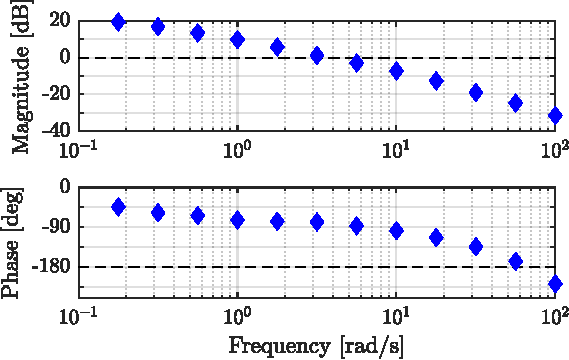
\includegraphics[keepaspectratio, scale=1.0]{contents/SystemIdentification/figure/crop-1018_manubode_in2fmea_7MPa.pdf}
        \caption{Frequency Response from Input to $\fmsr$ (\SI{7}{MPa})}
        \label{fig:crop-1018_manubode_in2fmea_7MPa}
\end{figure}
\begin{figure}[t]
    \centering
        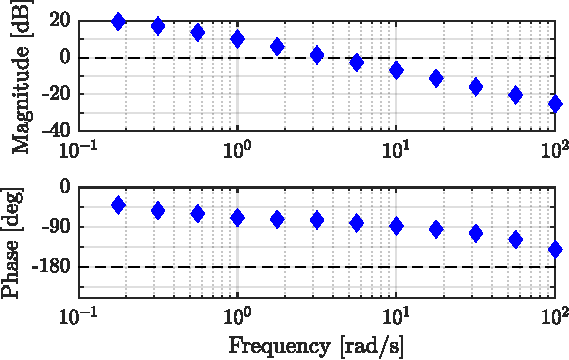
\includegraphics[keepaspectratio, scale=1.0]{contents/SystemIdentification/figure/crop-1018_manubode_in2fthr_7MPa.pdf}
        \caption{Frequency Response from Input to $\fthr$ (\SI{7}{MPa})}
        \label{fig:crop-1018_manubode_in2fthr_7MPa}
\end{figure}

\figname\ref{fig:crop-1018_manubode_in2fmea_7MPa}により,入力から実測出力$\fmsr$までのシステムは\eqnname\eqref{eq:tf_est_model}で表されるむだ時間を含む二次遅れ系であると判断した.
\begin{align}
    \label{eq:tf_est_model}
    \GinTofmsr = \frac{a}{(s+b)(s+c)}\mathrm{e}^{-ds}
\end{align}
\eqnname\eqref{eq:tf_est_model}の周波数応答が\figname\ref{fig:crop-1018_manubode_in2fmea_7MPa}と一致するように最小自乗法を用いて係数を決定すると,\eqnname\eqref{eq:tf_in2fmsr}となる.
\begin{align}
    \label{eq:tf_in2fmsr}
    \GinTofmsr = \frac{41.82}{(s+0.34)(s+130)}\mathrm{e}^{-0.016s}
\end{align}

同様に,入力から推力$\fthr$までの応答はむだ時間を含む一次遅れ系であるとし,その係数を求めると,\eqnname\eqref{eq:tf_in2fthr}となる.
\begin{align}
    \label{eq:tf_in2fthr}
    \GinTofthr = \frac{3.4}{s+0.34}\mathrm{e}^{-0.01s}
\end{align}
よって,推力$\fthr$から実測出力$\fmsr$までの伝達関数は\eqnname\eqref{eq:tf_in2fmsr}と\eqnname\eqref{eq:tf_in2fthr}より\eqnname\eqref{eq:tf_fthr2fmsr}となる.
\begin{align}
    \label{eq:tf_fthr2fmsr}
    \GfthrTofmsr = \frac{123}{s+130}\mathrm{e}^{-0.006s}
\end{align}
%\subsection{最小自乗法による伝達関数モデルの同定}
\section{位置までの同定}
\label{sec:位置までの同定}
バルブ入力からシリンダ位置までの応答のモデルの同定を行う.
本節ではシリンダ先端を拘束せず,自由に動く状態で同定を行う.

油圧シリンダにおける入力から位置までの同定は,線形な応答を前提に同定入力として正弦波の足し合わせを入力したもの\cite{ling2012system,zheng2009application}や,M系列による同定を行っているもの\cite{松本貴夢20166,松本貴夢2016},パラメータ同定を行っているもの\cite{前島祐三2011}がある.
本論文でははじめに,対象としている実験機のシリンダの応答の線形性を調べ,前節と同様に最小自乗法による周波数領域での同定,そしてM系列による同定を行う.
\subsection{線形性の検証}
バルブに正弦波入力を与え,位置の応答をフーリエ変換してピークを見ることにより線形性を調べる.
入力する正弦波の角速度は\ref{sec:線形性調査(力)}節と同様に\SI{0.1776}{rad/s}から\SI{100}{rad/s}までを対数上で等間隔に12等分したものを与える.

位置までの応答をフーリエ変換した結果を\figname\ref{fig:crop-pos_FFT}に示す.
\figname\ref{fig:crop-pos_FFT}において,入力した正弦波よりも低周波の部分でピークが立っており,応答は厳密には線形応答とは言えない.
本論文においてモデルを得たい領域は比較的低周波の領域であり,正弦波入力の角速度が\SI{50}{rad/s}以下の領域ではピークが大きくなく線形として扱える.
また先行研究において,線形システムとして同定を行った場合でも良い結果が得られていることなどより,本論文においても線形応答の対象としてシステムの同定を試みる.
\begin{figure}[t]
    \centering
        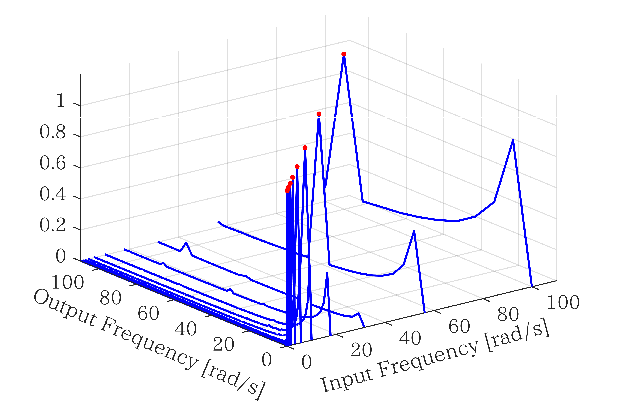
\includegraphics[keepaspectratio, scale=1.0]{contents/SystemIdentification/figure/crop-pos_FFT.pdf}
        \caption{FFT of Input to Position}
        \label{fig:crop-pos_FFT}
\end{figure}

\subsection{周波数領域における}
位置の応答までの周波数応答を\figname\ref{fig:pos_FR_mea-crop}に示す.
このときのポンプ圧力は\SI{7}{MPa}である.
\figname\ref{fig:pos_FR_mea-crop}より位置までの応答は積分器と一次遅れとむだ時間を含むシステムであると判断でき,最小自乗法により伝達関数モデルを求めると\eqnname\eqref{eq:tf_input2pos}となる.
\begin{align}
    \label{eq:tf_input2pos}
    \GinTopos = \frac{330}{s(s+60)}\mathrm{e}^{-0.002s}
\end{align}
\begin{figure}[t]
    \centering
        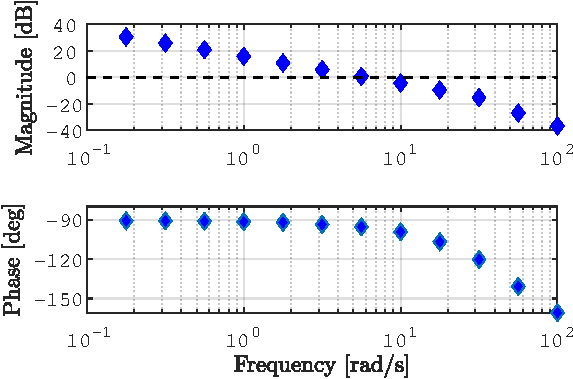
\includegraphics[keepaspectratio, scale=1.0]{contents/SystemIdentification/figure/pos_FR_mea-crop.pdf}
        \caption{Frequency Response from Input to Position}
        \label{fig:pos_FR_mea-crop}
\end{figure}

\clearpage
\begin{figure}[t]
    \centering
        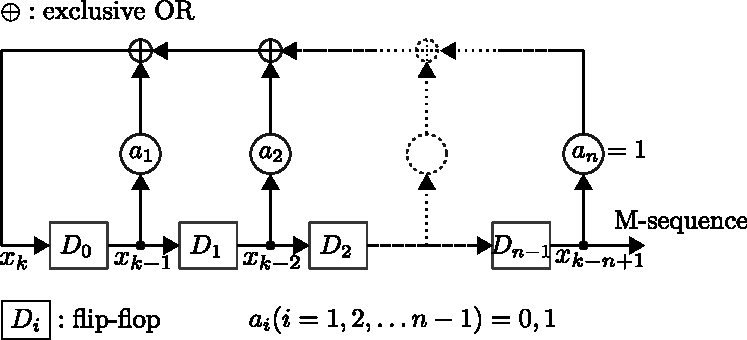
\includegraphics[keepaspectratio, scale=1.0]{contents/SystemIdentification/figure/Mseq.pdf}
        \caption{Generating Circuit of M-sequence}
        \label{fig:Mseq}
\end{figure}

\section{M系列入力を用いた時間領域におけるシステム同定}
\ref{sec:力までの同定}節および\ref{sec:位置までの同定}節では周波数領域で最小自乗法を適用することにより,伝達関数モデルを得た.
本来,対象とするシステムの正確なモデルを得るためには白色雑音を入力として用いることが望ましいが,現実的に白色雑音の適用は不可能であり,代わりとして擬似白色雑音を用いられる.
疑似白色雑音の一つがM系列と呼ばれる信号系列であり,信号の生成が比較的簡単であるためシステム同定の入力としてよく用いられている\cite{足立200909,柏木濶1998m}.
そこで本節では,同定入力にM系列を用いた場合のシステム同定について述べる.
\subsection{M系列の性質}
M系列とは,\figname\ref{fig:Mseq}に示す回路により生成される,0と1から構成される擬似白色雑音である.
\figname\ref{fig:Mseq}は$n$段のシフトレジスタの各段の値に係数$a_i$を乗じてフィードバックし,排他的論理和を適用させる構成になっている.
最初,シフトレジスタの各段には0または1の値が格納されており,全て0でなければその組み合わせは任意である.
これにより発生するM系列は以下の特徴をもつ\cite{吉谷清澄1971pn,近藤勝也2004m,柏木濶1981m}.
\begin{itemize}
    \item 周期系列であり,系列長は$p=2^n-1$である.(周期性)
    \item 1周期内に0は$2^{n-1}-1$個,1は$2^{n-1}$個存在する.(均一性)
    \item 1周期内において連続した$n$個の要素に着目したとき,そのビットパターンは全ての値が0である場合を除く全てのパターンが現れる.
    \item M系列中の1を+1に,0を-1に対応させると,自己相関関数$\phi_j$は\eqnname\eqref{eq:mseq-autocorec}のようになる.$j$は元の系列をシフトさせる数である.
    \begin{align}
        \label{eq:mseq-autocorec}
        \phi_j = 
        \begin{cases}
            \displaystyle
            1~&\mathrm{for}~j\equiv0~(\mathrm{mod}~p)\\
            \tfrac{-1}{p}~&\mathrm{for}~j\not\equiv0~(\mathrm{mod}~p)
        \end{cases}
    \end{align}
\end{itemize}
\subsection{システム同定(入力から力)}
\label{sec:Mseq_in2force}
バルブへの入力から力までの同定についてM系列を用いての同定を行う.
M系列を用いるさいのサンプリング周波数は,バンド幅の10倍程度に設定するのがよいため\cite{足立200909},\figname\ref{fig:crop-1018_manubode_in2fmea_7MPa}を参考にして,サンプリング時間\SI{0.2}{s}とし,シフトレジスタの個数$n$は8とした.

バルブへの入力と,力の入出力関係を\figname\ref{fig:1018Mseq_inputToFmea}に示す.
\figname\ref{fig:1018Mseq_inputToFmea}のうち,10$\sim$\SI{70}{s}を同定用のデータとして(\figname\ref{fig:1018Mseq_inputToFmea_10-70}),72$\sim$\SI{100}{s}を検証用データとして(\figname\ref{fig:1018Mseq_inputToFmea_72-100})用いる.

同定した伝達関数$\GinTofmsr$は,\eqnname\eqref{eq:tf_mseq_force}であり,分子第2項および分母第3項を微小として無視し整理すると,\eqnname\eqref{eq:tf_mseq_force_hosei}となる.
\begin{align}
    \label{eq:tf_mseq_force}
    \GinTofmsr&=\frac{4.193s+0.02265}{s^2 + 1.118s + 7.614\times 10^{-11}}\mathrm{e}^{-0.02s}\\
    \label{eq:tf_mseq_force_hosei} 
    \GinTofmsr&= \frac{4.19}{s+1.12}\mathrm{e}^{-0.02s}
\end{align}
\eqnname\eqref{eq:tf_mseq_force}および\eqnname\eqref{eq:tf_mseq_force_hosei}の応答と,\figname\ref{fig:1018Mseq_inputToFmea_72-100}の結果を比較すると,\figname\ref{fig:1018Mseq_compare}のようになる.
tf(w/o shaping)が\eqnname\eqref{eq:tf_mseq_force}の応答,tf(with shaping)が\eqnname\eqref{eq:tf_mseq_force_hosei}の応答である.
それぞれの横に書いてある数字はFit率であり,\eqnname\eqref{eq:fit}で算出される適合率の値である.
\begin{align}
    \label{eq:fit}
    \mathrm{Fit} =  \left( 1- \frac{\sqrt{\sum_{k=1}^N |\hat{y}(k)-y(k)|^2 }}{\sqrt{\sum_{k=1}^N |{y}(k)-\bar{y}|^2 }}\right) \times 100
\end{align}
ここで,$y(k)$は実際の出力,$\hat{y}(k)$はモデルの出力,$\bar{y}$は実際の出力の平均値である.
\figname\ref{fig:1018Mseq_compare}より,微小項を無視してもFit率がほぼ下がっていないので\eqnname\eqref{eq:tf_mseq_force_hosei}を同定結果として用いても問題ない.
よって\eqnname\eqref{eq:tf_mseq_force_hosei}をmodel TD:$\GTDforce$として扱う.
\begin{align}
    \label{eq:tf_GTDforce}
    \GTDforce = \frac{4.19}{s+1.12}\mathrm{e}^{-0.02s}
\end{align}
\begin{figure}[t]
    \centering
        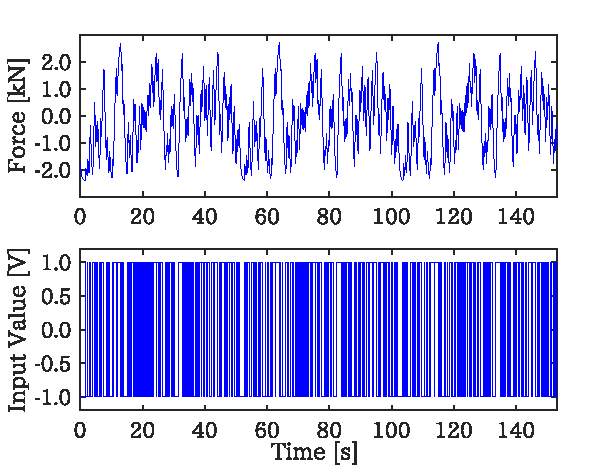
\includegraphics[keepaspectratio, scale=1.0]{contents/SystemIdentification/figure/1018Mseq_inputToFmea.pdf}
        \caption{Input and Output Data}
        \label{fig:1018Mseq_inputToFmea}
\end{figure}
\begin{figure}[t]
    \centering
        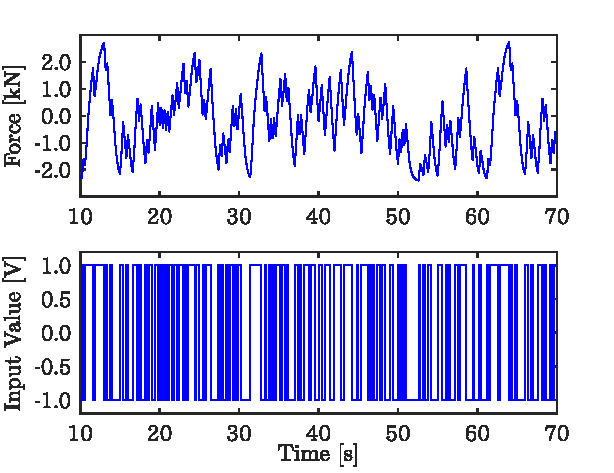
\includegraphics[keepaspectratio, scale=1.0]{contents/SystemIdentification/figure/1018Mseq_inputToFmea_10-70.pdf}
        \caption{Input and Output Data for System Identification}
        \label{fig:1018Mseq_inputToFmea_10-70}
\end{figure}
\begin{figure}[t]
    \centering
        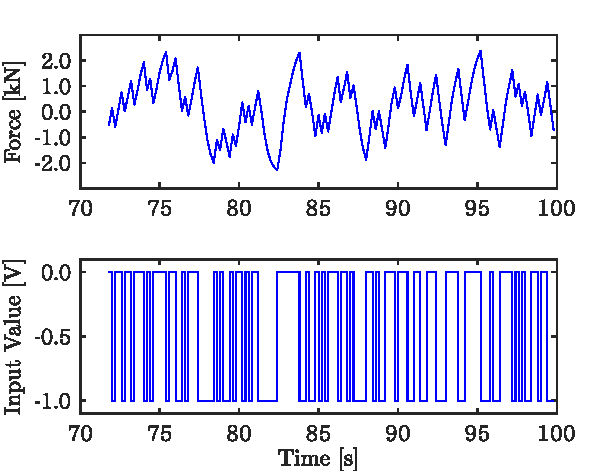
\includegraphics[keepaspectratio, scale=1.0]{contents/SystemIdentification/figure/1018Mseq_inputToFmea_72-100.pdf}
        \caption{Input and Output Data for Cross Validation}
        \label{fig:1018Mseq_inputToFmea_72-100}
\end{figure}
\begin{figure}[t]
    \centering
        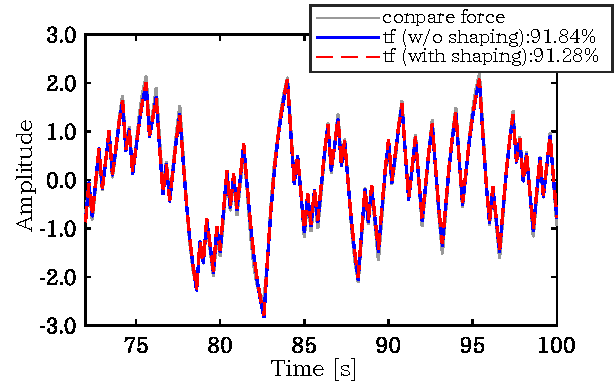
\includegraphics[keepaspectratio, scale=1.0]{contents/SystemIdentification/figure/1018Mseq_compare.pdf}
        \caption{Compare data}
        \label{fig:1018Mseq_compare}
\end{figure}

\clearpage
\subsection{システム同定(入力から位置)}
シリンダ先端を無負荷にした際の入力から位置までのシステムを同定する.
\figname\ref{fig:pos_FR_mea-crop}より,バルブへの入力から位置までには積分器が含まれている.
そのため,同定においては積分器が含まれることを前提としたシステム同定\cite{竹下侑2014積分器を有するシステムの同定について}を行う.
具体的な手法は以下のとおり.
\begin{itembox}[l]{積分器を有するシステムの同定手法}
    同定したいプラント$P(s)$に積分器がm個含まれているとき,その入出力関係をラプラス変換すると\eqnname\eqref{eq:sekibun_system}となる.
    \begin{align}
        \label{eq:sekibun_system}
        Y(s) = P(s)U(s) = \frac{1}{s^m}P'(s)U(s)
    \end{align}
    ここで,$P'(s)$は積分器を含まないシステムである.
    \eqnname\eqref{eq:sekibun_system}において${1}/{s^m}U(s)$を新たな入力$U_{\mathrm{new}}(s)$とし,入出力関係からm次トレンドを除去して同定を行うことにより$P'(s)$が求められる.
    $P'(s)$と$1/s^m$を合わせることにより,所望のシステムの伝達関数$P(s)$を得ることが可能である.
\end{itembox}
\ref{sec:Mseq_in2force}と同様に,シフトレジスタの数$n$を8,サンプリング周期\SI{0.2}{s}としたバルブへの入力と,位置の応答の入出力関係を\figname\ref{fig:crop-inputANDpos}に示す.
\figname\ref{fig:crop-inputANDpos}の入力に積分器を通した後の入出力関係は\figname\ref{fig:crop-inputANDpos_sekibun}となる.
\figname\ref{fig:crop-inputANDpos_sekibun}から1次トレンドを除去して同定したのち,積分器を付加した伝達関数$\GTDpos$は,
\begin{align}
    \label{eq:GTDpos}
    \GTDpos = \frac{1}{s}\frac{327.5}{s+48.32}\mathrm{e}^{-0.002s}
\end{align}
となる.
\eqnname\eqref{eq:GTDpos}の応答を実際の応答と比較すると,\figname\ref{fig:crop-pos_compare_mseq}となり,適合率\SI{97.25}{\%}での同定ができることがわかる.
これより,入力から位置までの同定には,積分器の存在を陽に考慮した同定が有効であると言える.
\begin{figure}[t]
    \centering
        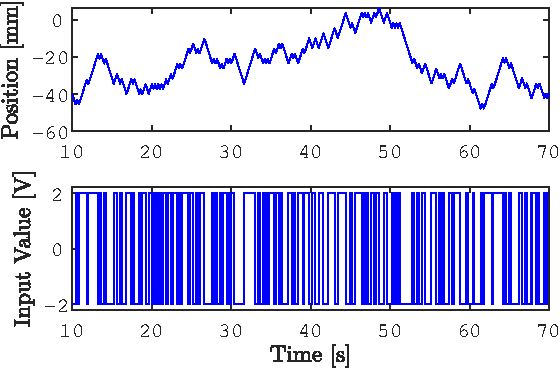
\includegraphics[keepaspectratio, scale=1.0]{contents/SystemIdentification/figure/crop-inputANDpos.pdf}
        \caption{Input and Output of Position}
        \label{fig:crop-inputANDpos}
\end{figure}
\begin{figure}[t]
    \centering
        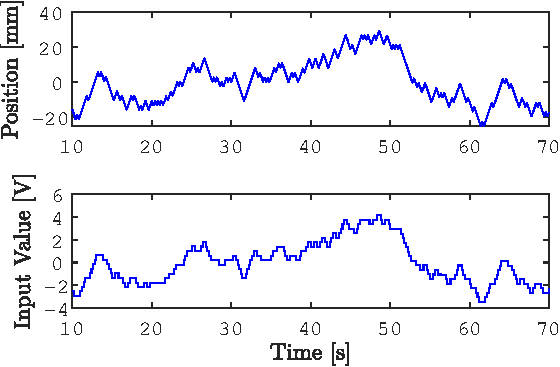
\includegraphics[keepaspectratio, scale=1.0]{contents/SystemIdentification/figure/crop-inputANDpos_sekibun.pdf}
        \caption{Integrated Input and Output of Position}
        \label{fig:crop-inputANDpos_sekibun}
\end{figure}
\begin{figure}[t]
    \centering
        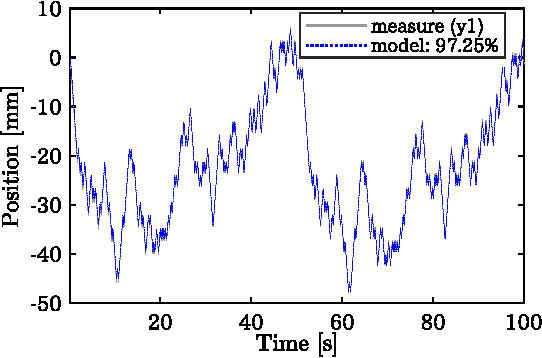
\includegraphics[keepaspectratio, scale=1.0]{contents/SystemIdentification/figure/crop-pos_compare_mseq.pdf}
        \caption{Cross Validation of Position}
        \label{fig:crop-pos_compare_mseq}
\end{figure}



































